\documentclass[letterpaper,12pt]{article}
\usepackage{fancyhdr}
\usepackage{amsmath}
\usepackage{amssymb}
\usepackage{bm}
\usepackage{numprint}
\usepackage[margin=1in]{geometry}
\usepackage{graphicx}
% Random packages from
% http://tex.stackexchange.com/questions/50070/landscape-figure-in-latex
% Necessary for sideways pictures
\usepackage{wrapfig}
\usepackage{lscape}
\usepackage{rotating}
\usepackage{epstopdf}
\usepackage{tablefootnote}
% for word wrap verbatim
\usepackage{listings}
\lstset{
   breaklines=true,
   basicstyle=\ttfamily}
% \pagestyle{fancy}
% \lhead{Jesse Mu}
% \rhead{CSCI339 Term Project}
% One more .. since we're in the abbreviated subdir
\graphicspath{ {../../figures/abbreviated/} {../../figures/} }



\begin{document}

\title{Cluster Analysis: Identifying Parkinson's Disease Subtypes}
\maketitle

\section{Preprocessing}

\subsection{Dataset Description}
951 subjects, 145 metrics, collected 15-4-2012 from Pablo Martinez Mart\'in. Only
19 features used for clustering and/or interpretation.  50 subjects with
missing values of the features to be used in clustering (brought down to 901).
Imputation may be a good idea later on.

\subsection{Selected Features}

Combination of non-motor scale (NMS) symptoms and standard motor symptoms.

\begin{table}[h]
  \centering
  \begin{tabular}{l|l|l|l}
    Name & Type & Format & Description \\
    \hline
    nms\_d1 & byte & \%8.0g & cardiovascular \\
    nms\_d2 & byte & \%8.0g & sleep/fatigue \\
    nms\_d3 & byte & \%8.0g & mood/cognition \\
    nms\_d4 & byte & \%8.0g & percep/hallucinations \\
    nms\_d5 & byte & \%8.0g & attention/memory \\
    nms\_d6 & byte & \%8.0g & gastrointestinal \\
    nms\_d7 & byte & \%8.0g & urinary \\
    nms\_d8 & byte & \%8.0g & sexual function \\
    nms\_d9 & byte & \%8.0g & miscellaneous \\
    tremor & float & \%9.0g & tremor \\
    bradykin & float & \%9.0g & bradykinesia\tablefootnote{Impaired ability to
    adjust the body's position.} \\
    rigidity & float & \%9.0g & rigidity \\
    axial & float & \%9.0g & axial\tablefootnote{Issues affecting the middle of
    the body.} \\
    pigd & float & \%9.0g & postural instability and gait difficulty \\
  \end{tabular}
  \caption{Selected Features and Details}
  \label{tab:selected-features}
\end{table}

\begin{table}[h]
  \centering
  \begin{tabular}{l|l|l|l}
  Name  &       $\mu$ & $\sigma$ & min-max \\
         \hline
nms\_d1&   1.73&  3.35&   0-24 \\
nms\_d2&   8.75&  8.70&   0-48 \\
nms\_d3&   8.68& 11.55&   0-60 \\
nms\_d4&   1.64&  3.86&   0-33 \\
nms\_d5&   5.42&  7.43&   0-36 \\
nms\_d6&   5.53&  6.79&   0-36 \\
nms\_d7&   8.08&  8.94&   0-36 \\
nms\_d8&   3.52&  5.97&   0-24 \\
nms\_d9&   7.13&  7.79&   0-48 \\
tremor&   2.59&  2.58&   0-12 \\
bradykin& 2.40&  1.41&   0-6 \\
rigidity& 2.24&  1.36&   0-6 \\
axial&    3.25&  2.68&   0-12 \\
pigd&     3.31&  2.71&   0-12 \\
  \end{tabular}
  \caption{Descriptive Statistics}
  \label{tab:descriptive-statistics}
\end{table}

\section{$k$-means}

$k$-means clustering with $k = 4$ was tried. $k = 2, 3$ provided models that
were too simplistic. $k = 5$ did not provide any new information, but rather
just fragmented existing groups.

\begin{table}[h]
  \centering
  \caption{Cluster statistics}
  \label{tab:cluster_stats}
  \begin{tabular}{l|l}
    Cluster & $n$ \\
    \hline
    1 & 79 \\
    2 & 394 \\
    3 & 275 \\
    4 & 153 \\
  \end{tabular}
\end{table}

\subsection{Decision tree}
\begin{table}[h]
  \centering
  \begin{tabular}{l|l|l|l|l|l}
    $k$ & CP\tablefootnote{Complexity Parameter} & CV Xerror\tablefootnote{10-fold cross
    validation} & Root Feature &
    Root Error & Figure \\
    \hline
    4 & 0.0100 & 0.255 & pigd $<$ 2.5 & 0.563 & Figure~\ref{fig:kmeans-dtree-4} \\
  \end{tabular}
  \caption{$k$-kmeans decision trees statistics}
  \label{tab:k-means-dtrees}
\end{table}

\begin{figure}[h]
  \centering
  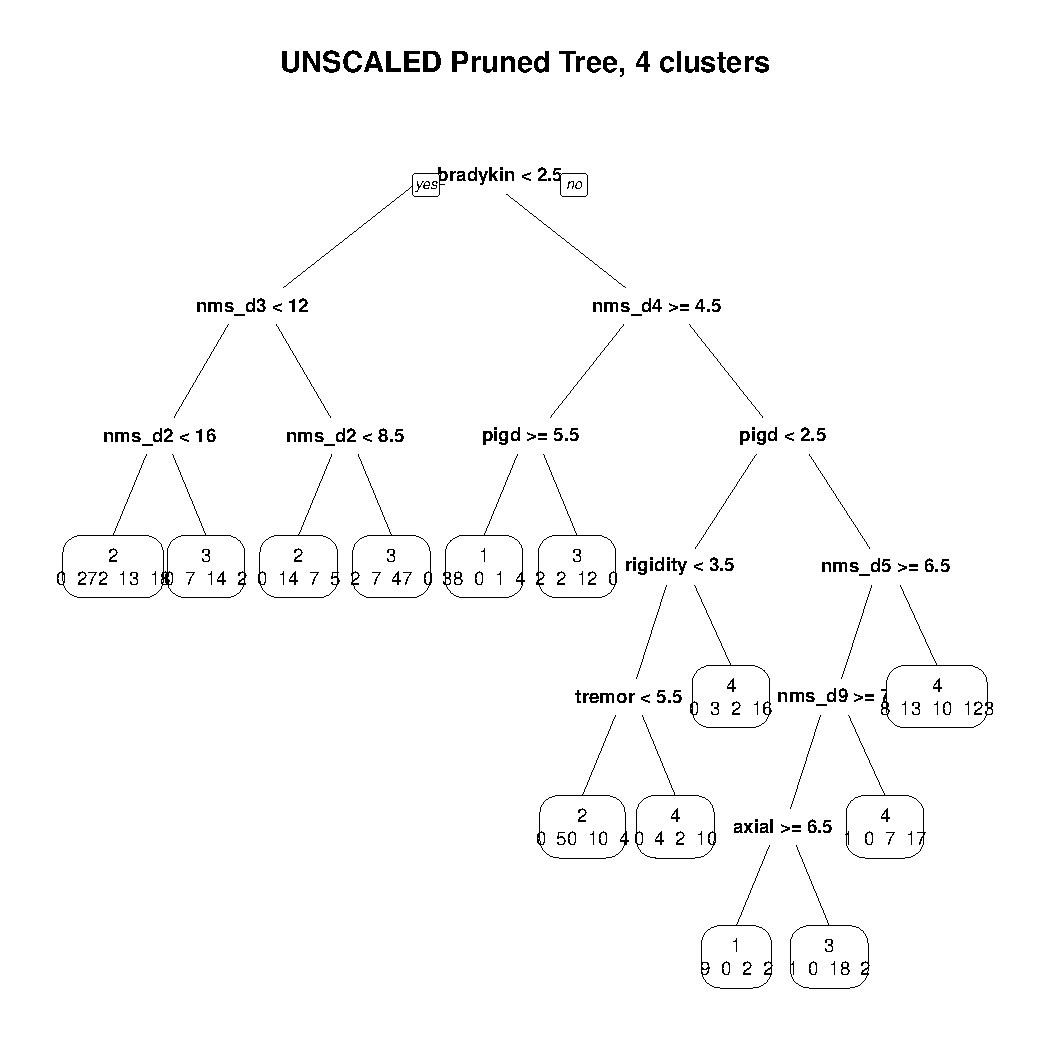
\includegraphics[width=\linewidth]{dtree-kmeans-pruned-unscaled-4.pdf}
  \caption{Decision Tree from $k$-means clustering, 4 clusters}
  \label{fig:kmeans-dtree-4}
\end{figure}

\subsection{Interpretation of Clusters}

\subsubsection{Cluster summaries}

Available in Figure~\ref{fig:kmeans-summaries-4}. Error bar is standard error.

\begin{figure}[h]
  \centering
  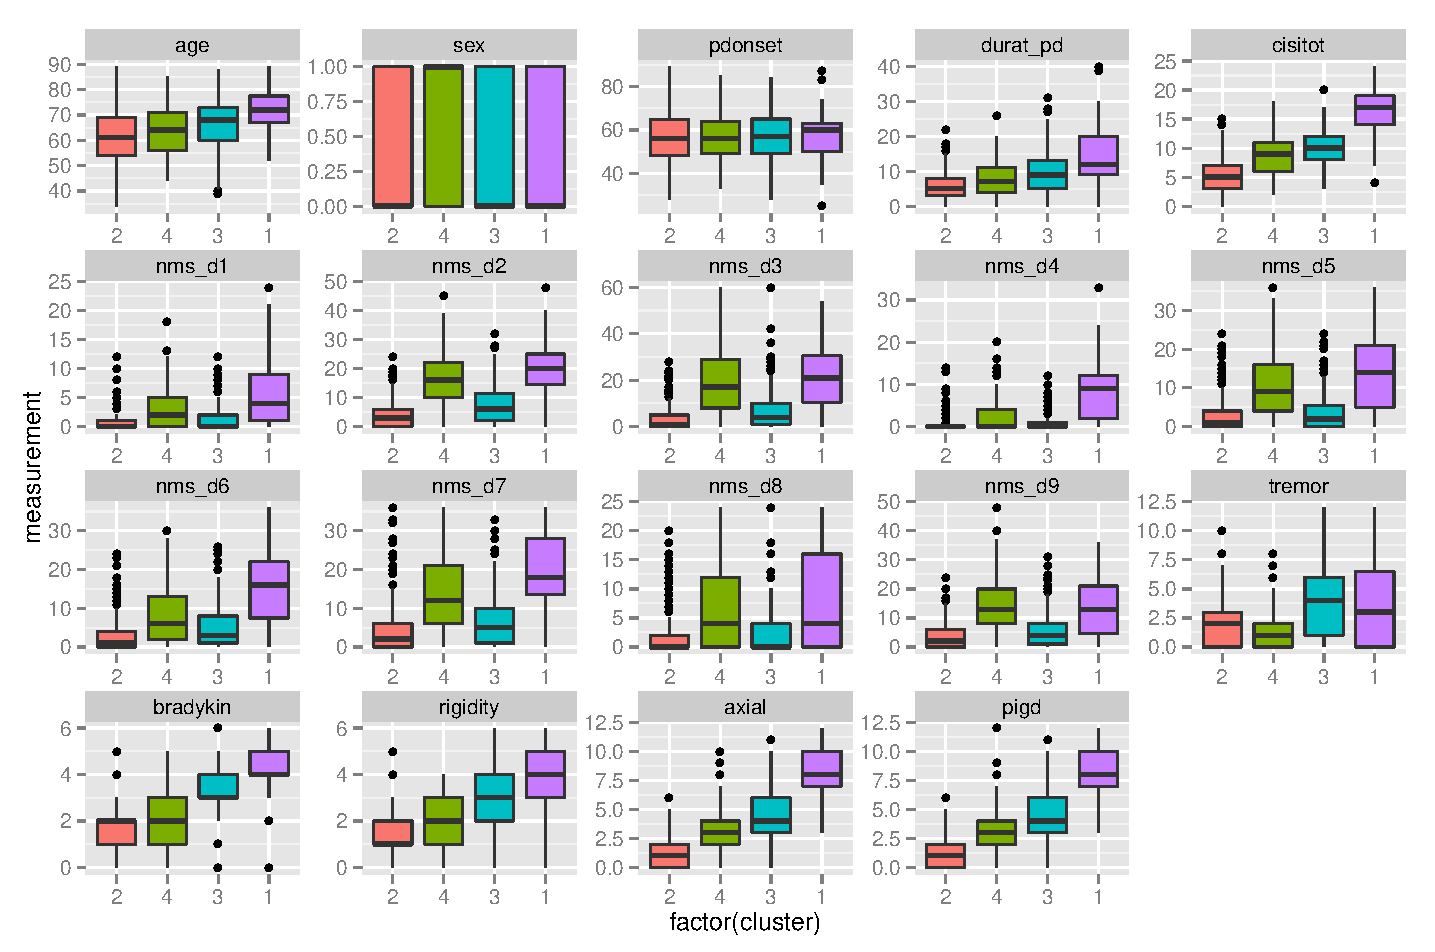
\includegraphics[width=\linewidth]{kmeans-summaries-4.pdf}
  \caption{Cluster Summaries, $k = 4$}
  \label{fig:kmeans-summaries-4}
\end{figure}

\subsubsection{Interpretation}

\subsubsection{Statistical Significance Tests, $k = 4$}
Using one-way ANOVA for multiple means, we reject the null
hypothesis that the means are the same with $p < 0.05$ for every variable
\emph{except} \texttt{pdonset}.

Post-hoc analysis using Tukey's HSD:
\begin{verbatim}
age insignificant differences:
         diff         lwr        upr        p adj
4-3 -2.271990  -4.7160927  0.1721117 7.920343e-02
sex insignificant differences:
           diff        lwr        upr     p adj
2-1 -0.09275204 -0.2454183 0.05991417 0.4000134
3-1 -0.14660529 -0.3046921 0.01148156 0.0803067
4-1  0.04757177 -0.1240051 0.21914864 0.8917054
3-2 -0.05385325 -0.1511666 0.04346014 0.4843788
pdonset insignificant differences:
           diff       lwr      upr     p adj
2-1 -0.90162565 -4.302019 2.498768 0.9037828
3-1 -0.05040276 -3.571532 3.470727 0.9999820
4-1 -0.53727145 -4.358869 3.284326 0.9837825
3-2  0.85122289 -1.316276 3.018722 0.7431486
4-2  0.36435420 -2.263251 2.991959 0.9844187
4-3 -0.48686869 -3.268952 2.295214 0.9695444
nms_d1 insignificant differences:
          diff         lwr       upr        p adj
3-2  0.5565021 -0.01586385  1.128868 6.018674e-02
nms_d3 insignificant differences:
          diff        lwr        upr       p adj
4-1  -1.192024  -4.493510   2.109461 0.789133802
nms_d4 insignificant differences:
          diff        lwr       upr        p adj
3-2  0.2951915 -0.3318339  0.922217 6.195406e-01
nms_d5 insignificant differences:
           diff         lwr       upr        p adj
3-2   0.7841071  -0.4814825  2.049697 0.3821565990
nms_d8 insignificant differences:
          diff       lwr      upr     p adj
4-1 -0.9010507 -2.846119 1.044017 0.6318563
3-2  0.7255838 -0.377602 1.828770 0.3280035
nms_d9 insignificant differences:
          diff         lwr       upr       p adj
4-1  0.7048896  -1.6510530  3.060832 0.867951568
tremor insignificant differences:
          diff       lwr        upr      p adj
3-1 -0.2662831 -1.064520 0.53195417 0.82613187
4-2 -0.5667198 -1.162396 0.02895624 0.06895758
rigidity insignificant differences:
          diff         lwr        upr        p adj
4-2  0.2310142 -0.03536748  0.4973959 1.153952e-01
\end{verbatim}

\subsubsection{Ranked Features by Information Gain}

\begin{table}[h]
  \centering
  \caption{Features ranked by information gain}
  \label{tab:info_gain}
  \begin{tabular}{l|l}
    variable & information gain \\
    \hline
    axial      & 0.20640691 \\
    cisitot      & 0.20008571 \\
    pigd      & 0.18193982 \\
    nms\_d2      & 0.13178572 \\
    nms\_d9      & 0.12116024 \\
    bradykin      & 0.11966097 \\
    nms\_d3      & 0.09421859 \\
    rigidity      & 0.09260628 \\
    nms\_d5      & 0.07579997 \\
    nms\_d4      & 0.07438784 \\
    nms\_d6      & 0.06620599 \\
    nms\_d7      & 0.05574956 \\
    nms\_d1      & 0.05509838 \\
    tremor      & 0.04140473 \\
    nms\_d8      & 0.03786173 \\
    durat\_pd      & 0.02794420 \\
    age      & 0.00000000 \\
    sex      & 0.00000000 \\
    pdonset      & 0.00000000 \\
  \end{tabular}
\end{table}

\subsubsection{Correlation Plots}

Figure~\ref{fig:corrplots}.

\begin{figure}[h]
  \centering
  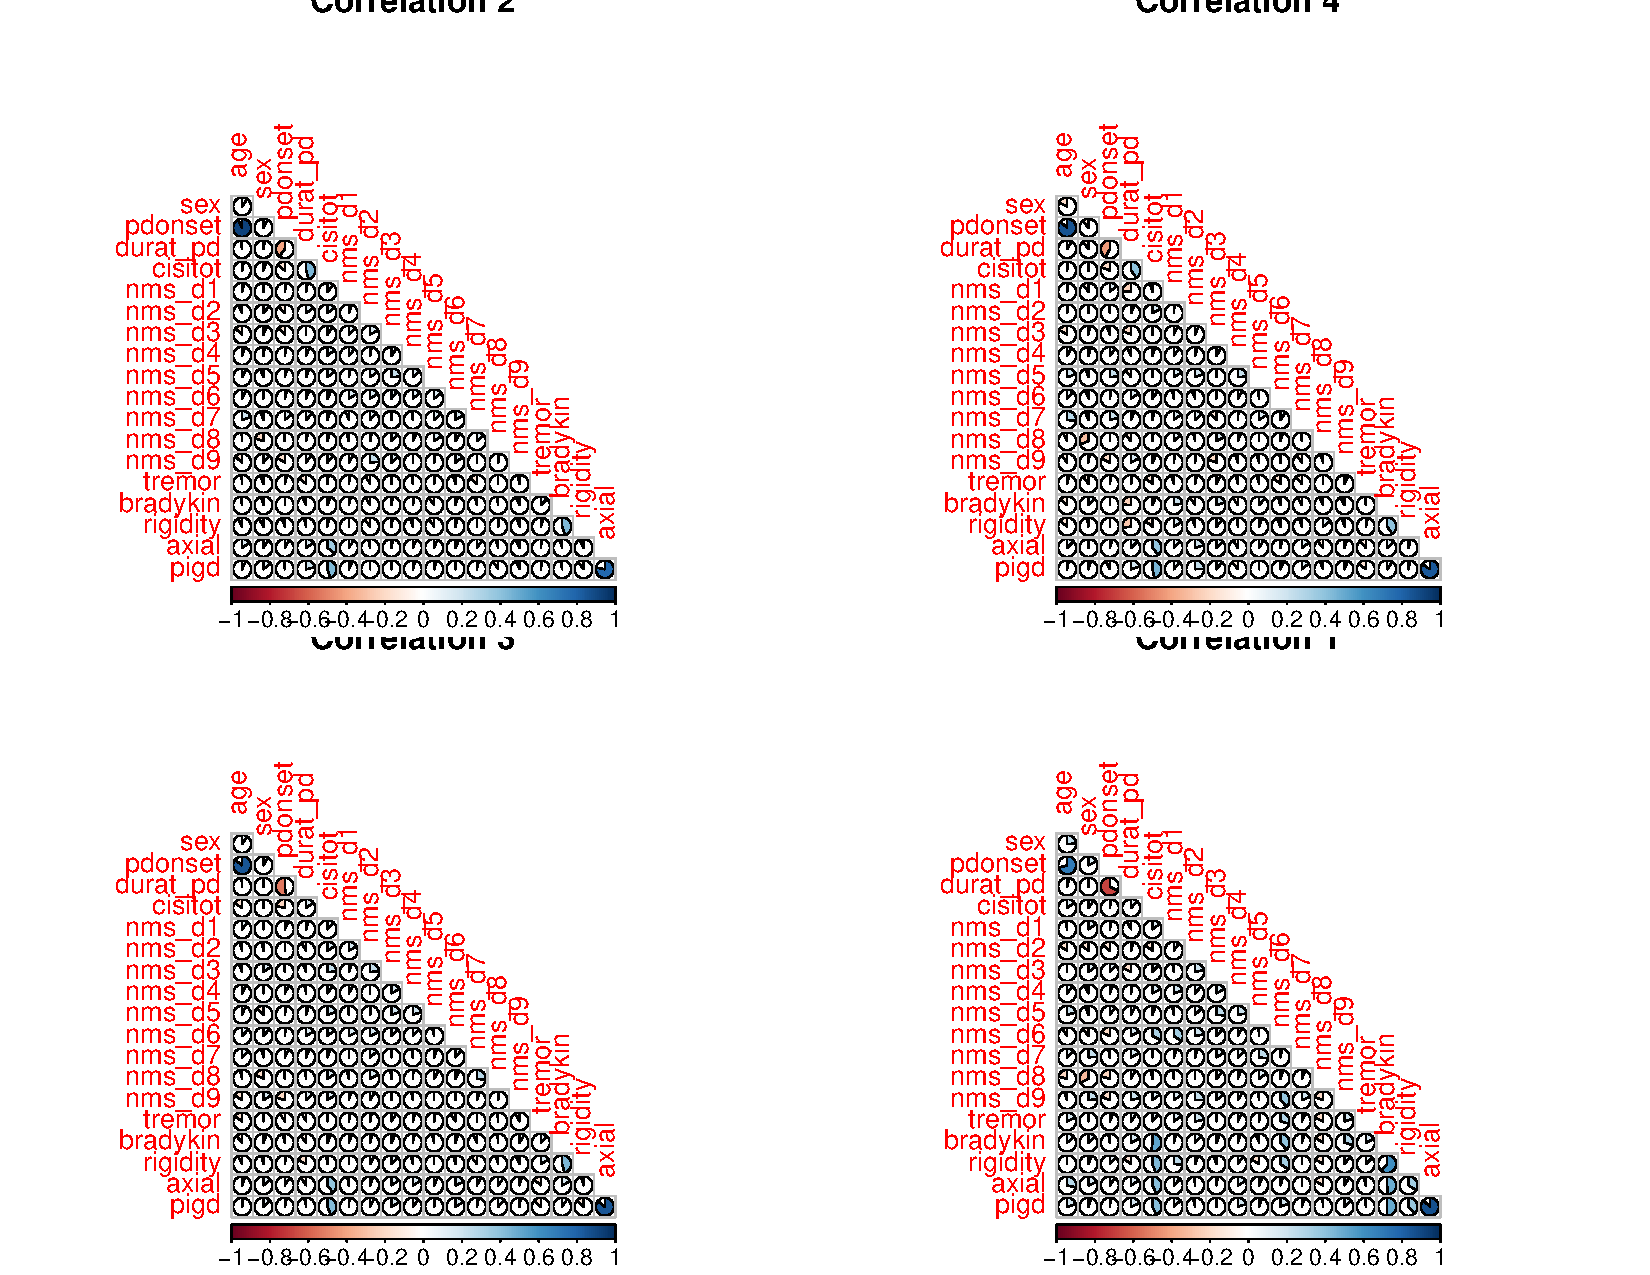
\includegraphics[width=\linewidth]{corrplots.pdf}
  \caption{Correlation plots}
  \label{fig:corrplots}
\end{figure}

\subsubsection{Bradykinesia and rigidity}

Figures~\ref{fig:bradykin-cisitot} and~\ref{fig:rigidity-cisitot}

\begin{figure}[h]
  \centering
  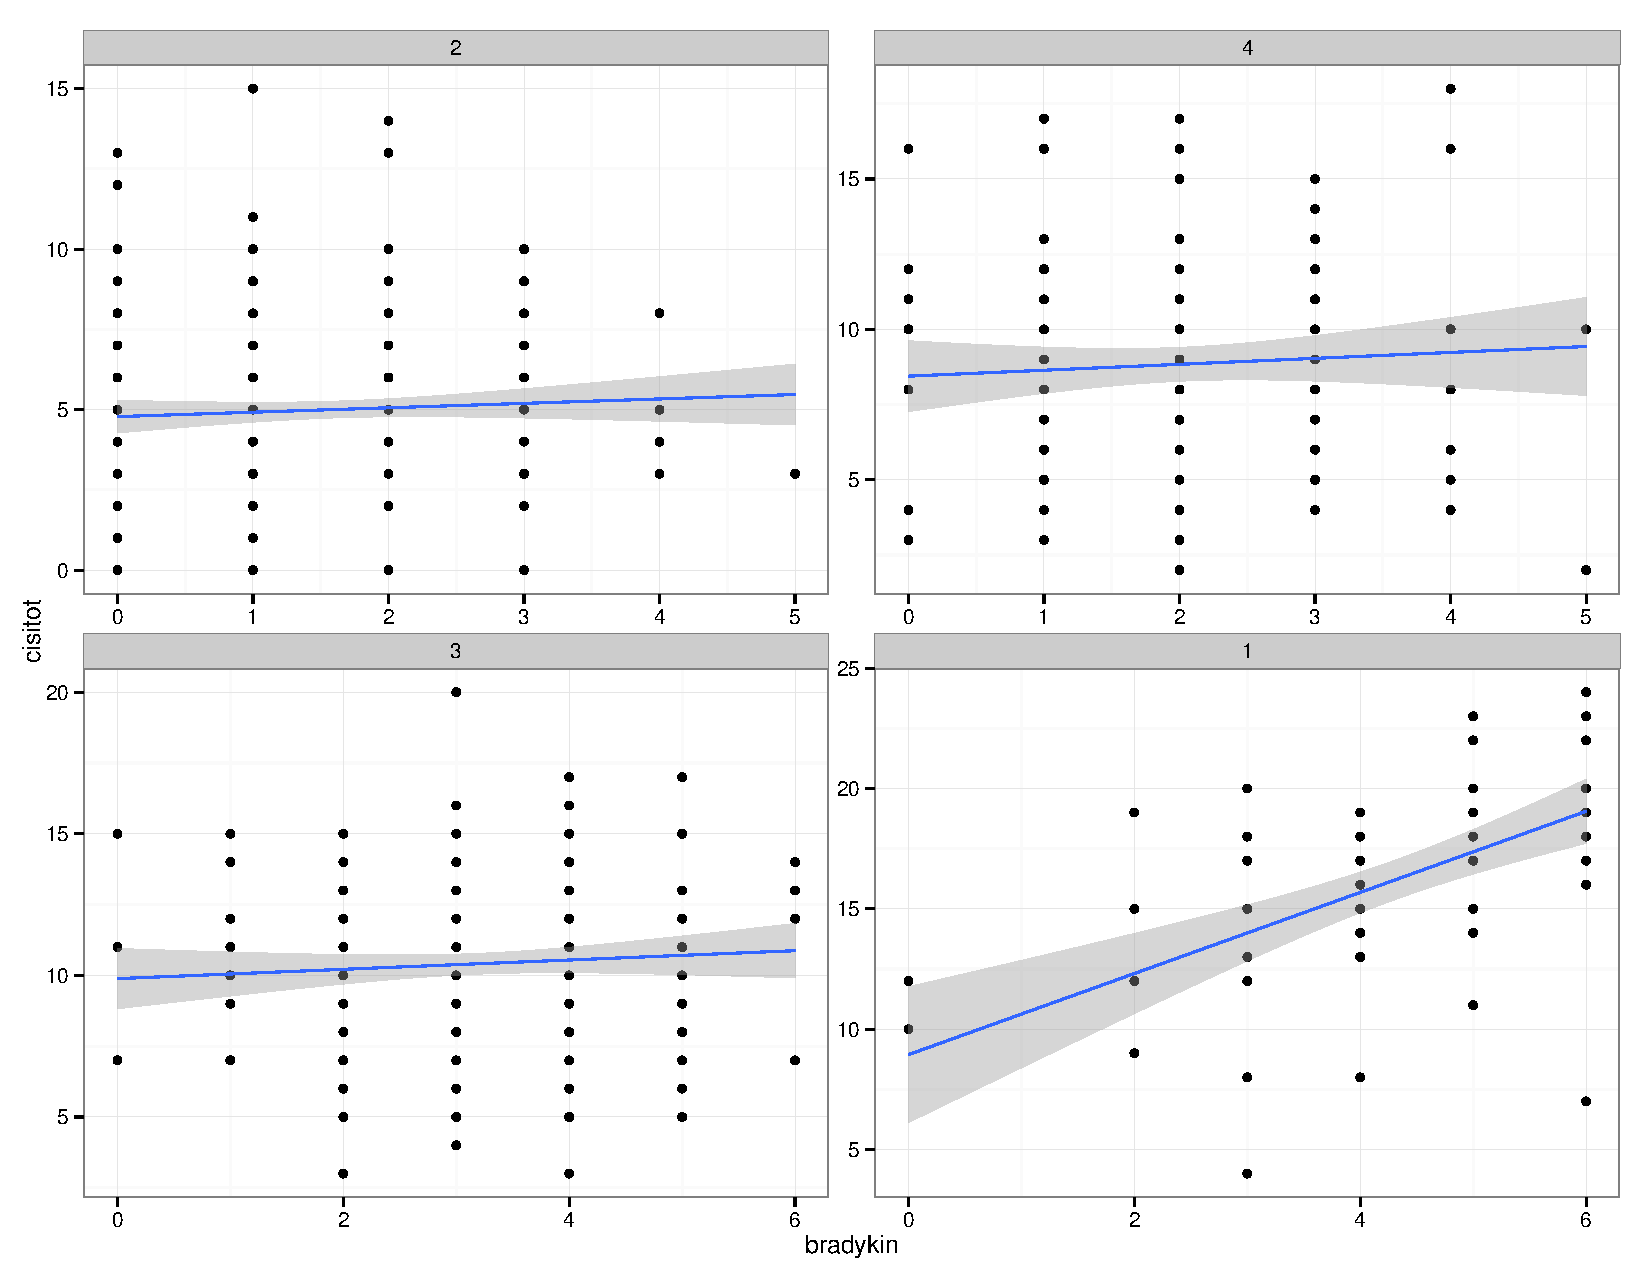
\includegraphics[width=\linewidth]{bradykin-cisitot.pdf}
  \caption{Relationship between bradykinesia and cisitot}
  \label{fig:bradykin-cisitot}
\end{figure}

\begin{figure}[h]
  \centering
  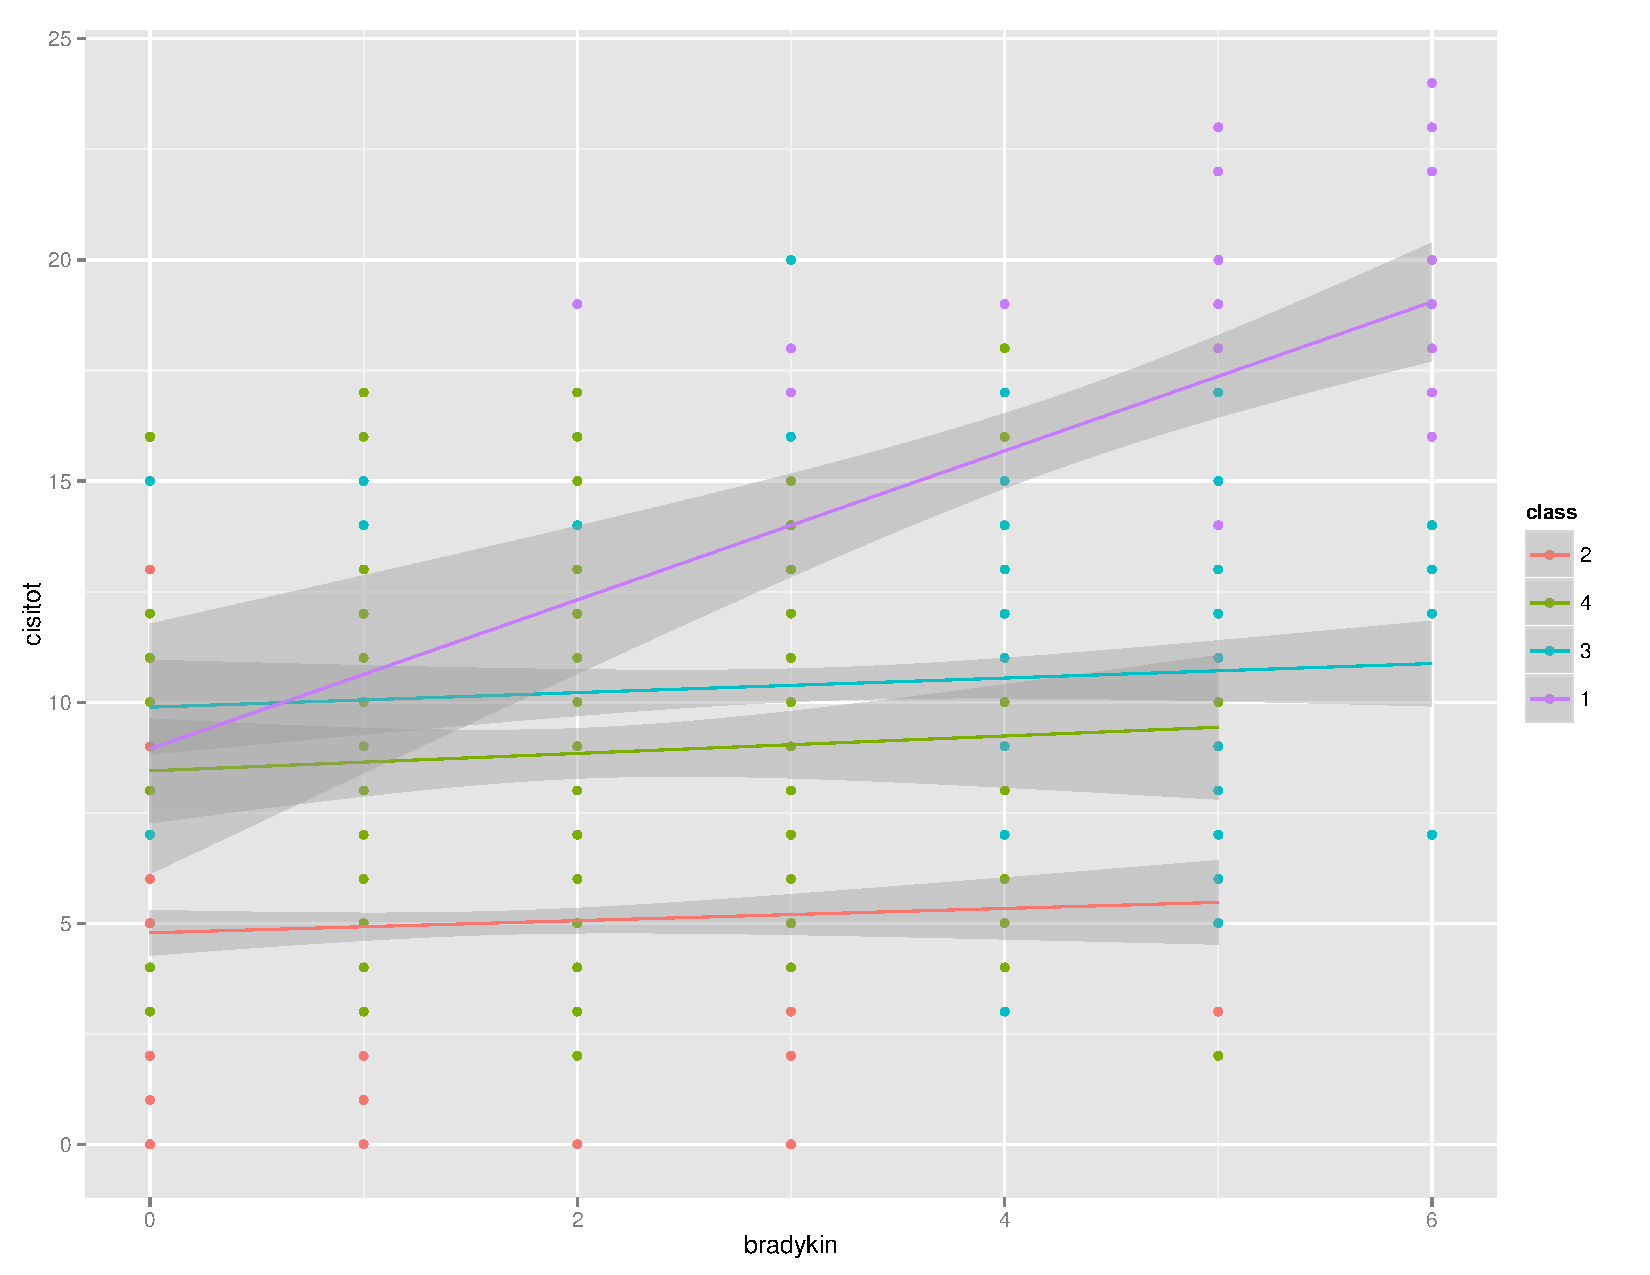
\includegraphics[width=\linewidth]{bradykin-cisitot-condensed.pdf}
  \caption{Relationship between bradykinesia and cisitot (condensed)}
  \label{fig:bradykin-cisitot-condensed}
\end{figure}

\begin{figure}[h]
  \centering
  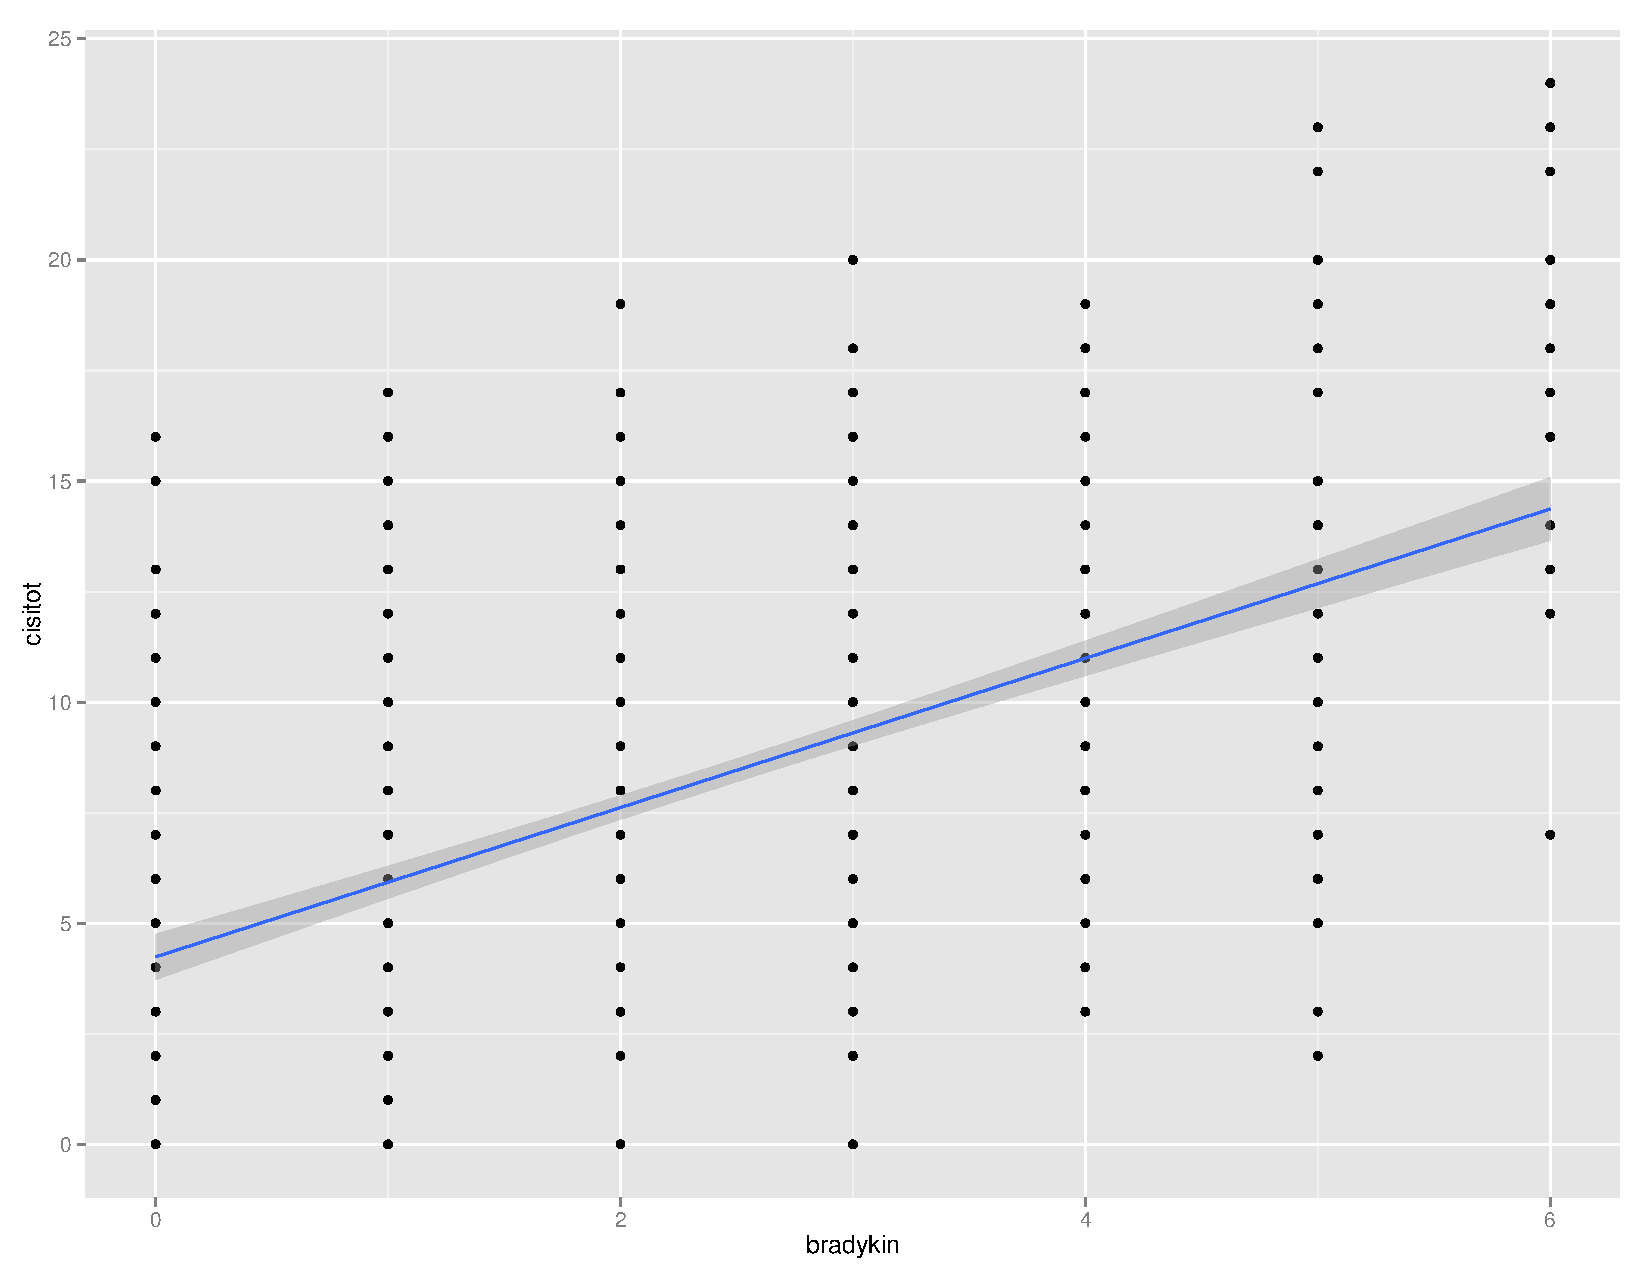
\includegraphics[width=\linewidth]{bradykin-cisitot-all.pdf}
  \caption{Relationship between bradykinesia and cisitot (entire data)}
  \label{fig:bradykin-cisitot-all}
\end{figure}

\begin{figure}[h]
  \centering
  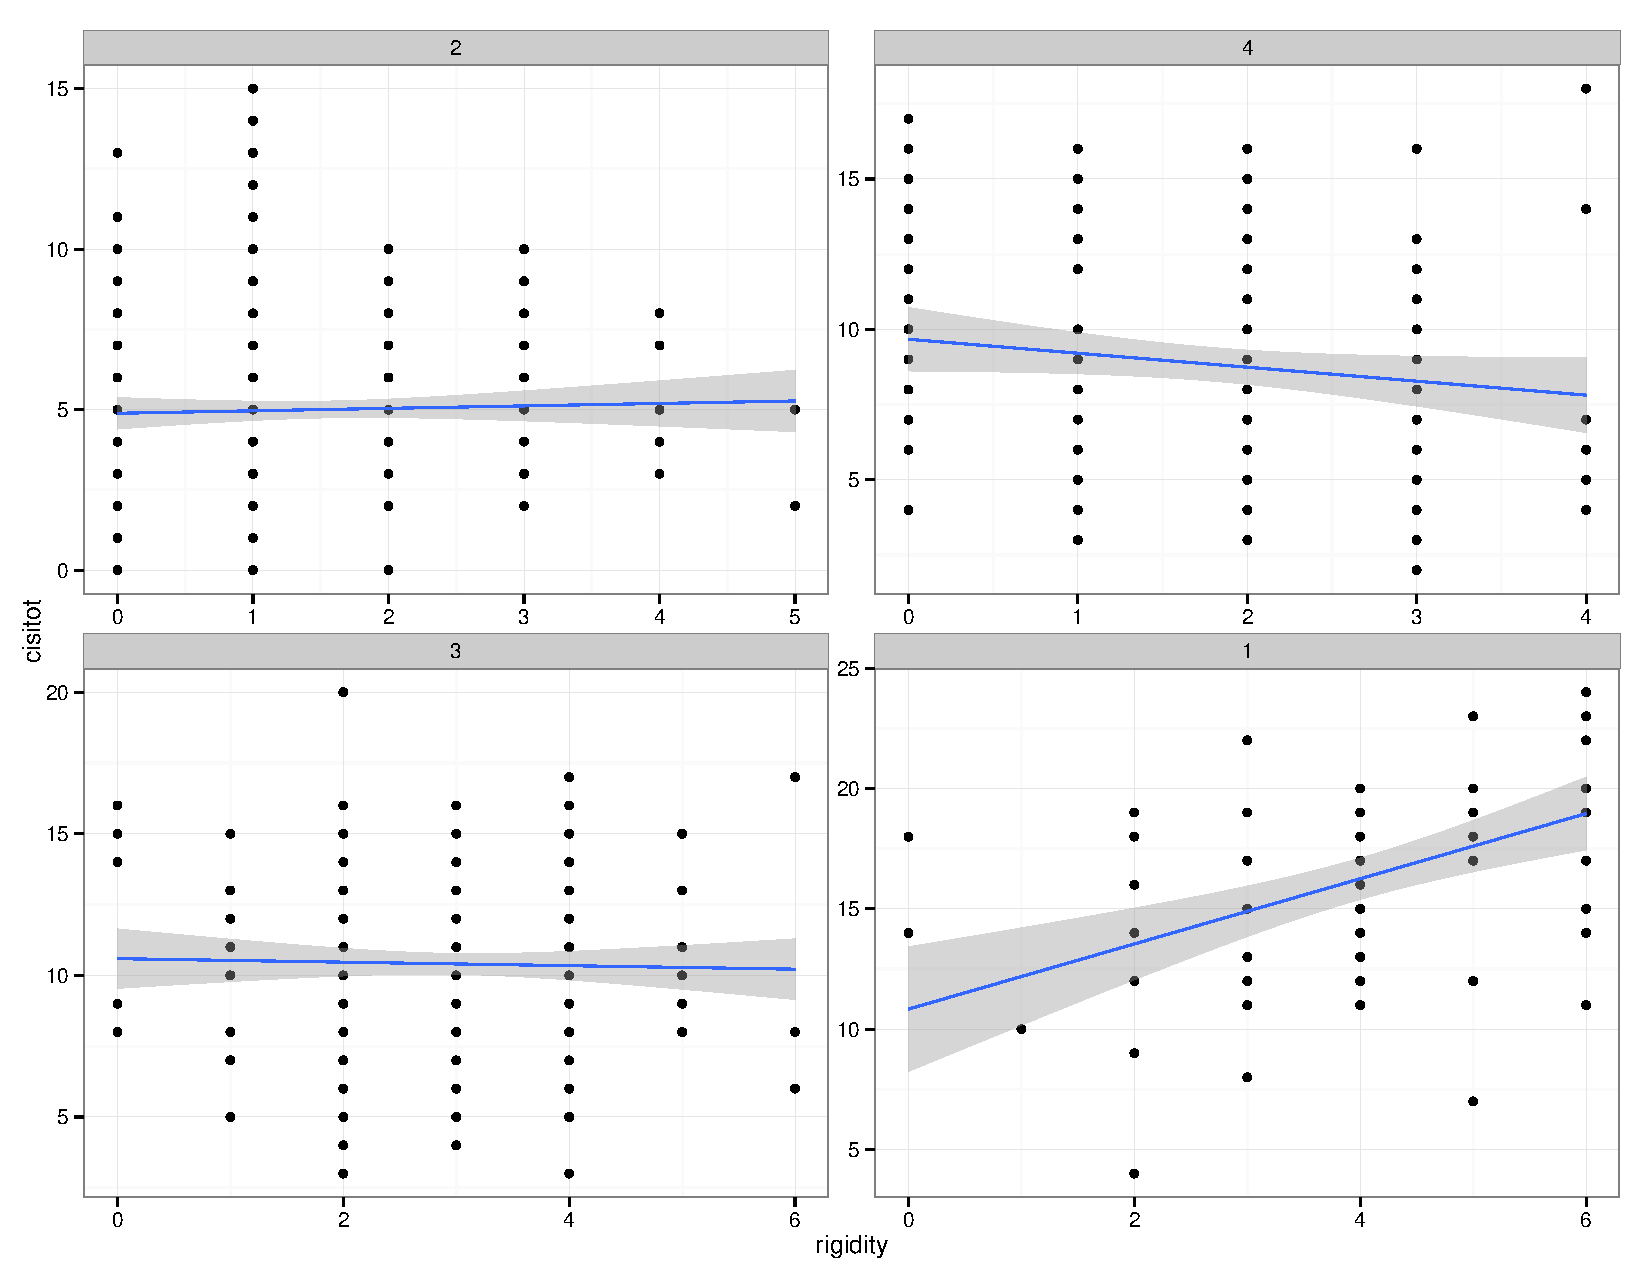
\includegraphics[width=\linewidth]{rigidity-cisitot.pdf}
  \caption{Similar relationship between rigidity and cisitot}
  \label{fig:rigidity-cisitot}
\end{figure}

\section{Other Work}

\subsection{Bayesian Networks}

In Figure~\ref{fig:bnets}. Structure is too sparse, need to discretize or use
some kind of regularization (e.g. a lasso)

\begin{figure}[h]
  \centering
  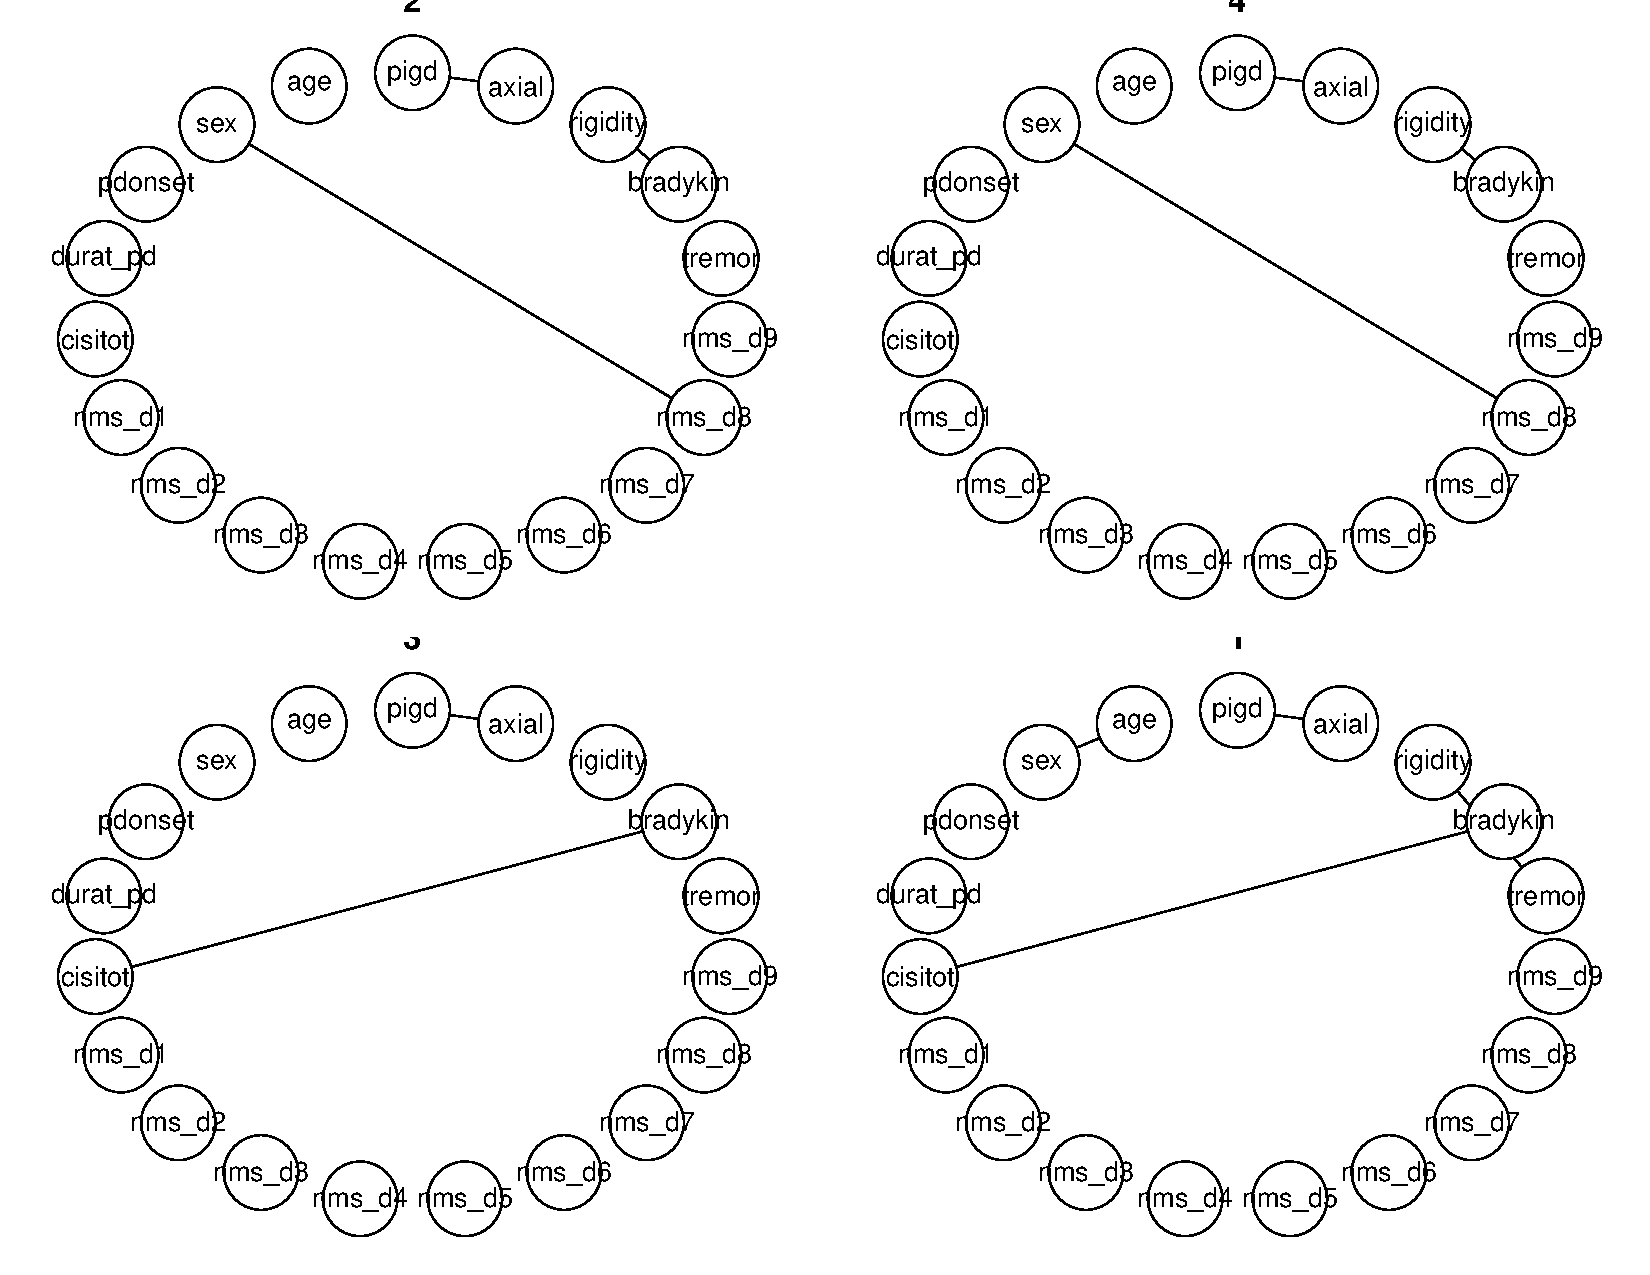
\includegraphics[width=0.8\linewidth]{bnets.pdf}
  \caption{Bayesian Networks}
  \label{fig:bnets}
\end{figure}

\end{document}
